\documentclass{article}
\usepackage{hyperref}
\usepackage{graphicx, amsmath, amssymb, bm, scrextend, titling, physics, bbm, url}
\usepackage{hyperref}
\setlength\parindent{0pt}
\usepackage{geometry}


\title{Stochastic Invasion of a VoC and Onward Transmission}

\date{March 2021}


\begin{document}
\maketitle

We cross-check the results of our Gillespie simulation with analytic results for a continuous-time multi-type branching process model with immigration that models the stochastic invasion of a variant strain into a heterogenous population. \\

\subsection{Model Description}
We consider the disease dynamics of an invading Variant of Concern (VoC) into a population that has had previous exposure to a wild-type strain and has undergone an incomplete vaccination program with 3 different vaccines (Pfizer (Pf), Astra-Zeneca (AZ) and a new, updated vaccine (N)). The novel strain is assumed to exhibit some resistance to both infection-acquired and vaccine-acquired immunity. We model the invasion and early transmission of this new strain using a multi-type branching process model \cite{dorman2004garden}. \\ 

We consider an epidemic in which the population is divided into 16 types, namely, 8 exposed types $E_{d, v}$ and 8 infectious types $I_{d, v}$ where $d \in \{\mathrm{sus, rec}\}$ denotes whether an individual is susceptible to the current wild-type strain of COVID or has been infected previously and has recovered,  and where $v\in\{ \mathrm{U, AZ, Pf, N}\}$ denotes whether an individual is unvaccinated or has been vaccinated with the Astra-Zeneca, Pfizer or new vaccine, respectively. We order the types in our model combinatorially so that types 1-8 correspond to exposed cases and types 9-16 correspond to infectious cases. Exposed cases become infectious at a constant rate $\sigma$ and infectious cases have a constant recovery rate $\gamma$. \\

Each type of individual has a relative susceptibility to the VoC determined by their previous exposure to other variants and by their vaccination status. In our model this is interpreted as each infectious type having equal transmissibility $\beta$ and exerting a force of infection on susceptible individuals of type $j \, (1 \leq j \leq 8)$ given by $\beta_j = c_j \beta$, where the constant $c_j$ scales $\beta$ by the relative proportions of type $j$ in the population and by the relative susceptibility of each type to the VoC. At each infection event in our model an infectious individual is replaced by an exposed case of type $j$ and an identical copy of itself. For convenience, we denote the lifetime of a particle of a case of type $i$ by $\omega_i = \sigma$ for  $1 \leq i \leq 8$ and by $\omega_i = \sum_{j=0}^8 \beta_j + \gamma$ for $9 \leq i \leq 16$. The generating function for the offspring distribution of this process, the distribution of the number of cases of each type produced by a case of type $i$ at a single event, is given by:


\begin{equation} \label{offspring}
P_i(s) =  \begin{cases}
 s_{i+8} \quad \text{for} \, 1 \leq i \leq 8 \\
\\
\frac{\sum_{j=0}^8 \beta_j s_j s_i}{\omega_i} + \frac{\gamma}{\omega_i} \quad \text{for} \, 9 \leq i \leq 16 
\end{cases}
\end{equation}


where $s = (s_i)_{i=1}^{16}$ is a vector of length 16 whose components correspond to each different type of infected individual. In our model, we initially consider a process that starts with a single case of type $i$ at time $t=0$ and no other cases, and consider the total number of cases of all types at time $t$, which we denote by $Y_i(t)$ for $ (1 \leq i \leq 16)$.  For each $1 \leq i \leq 16$, the random variable $Y_i(t)$ has generating function $Q_i(t, s) = \sum_{n=0}^\infty{\mathrm{Pr}}(Y_i(t) = n)s^n$. Since $s$ is a vector, $s^n$ denotes the product $s_1^{n_1} \cdot \dots \cdot s_{16}^{n_{16}}$, where $n_i$ is the number of cases of type $i$ and $n = \sum_i n_i$. \\ 

We obtain expressions for the $Q_i(t)$ by solving:
\begin{equation}
    \frac{\partial Q_i(t, s)}{\partial t} = -\omega_i[Q_i(t, s) - P_i(Q)], \quad Q(0, s) = s \label{Qeq}
\end{equation}
where $Q(t, s) = [Q_i(t, s)]_{i=1}^{16}$ is a vector. Setting $s=0$ gives the vector  $q(t) = Q(0, s)$ of extinction probabilities for a process starting with a single particle of type $i$. \\

We then consider a process that begins with no cases of any type, but that allows immigration of exposed cases of type $i$ at a rate $\eta_i$ and write $\eta = \sum_i \eta_i$. The total number of particles of all types at time $t$ for this process is denoted by $Z(t)$ and has the generating function $R(t, s) = \sum_{n=0}^\infty {\mathrm{Pr}}(Z(t) = n)s^n$, which we obtain by solving:
\begin{equation}
    \frac{\partial R(t, s)}{\partial t} = -\eta R(t, s) + \sum_{i=0}^{16} \eta_i R(t, s)Q_i(t, s), \quad \text{subject to }\, R(0, s) = 1 \label{Req}
\end{equation}
Setting $s=0$ as before, we find the probability of zero cases of any type at time $r(t) = R(t, 0)$. This should no longer be interpreted as a probability that a strain goes extinct, as immigration allows new cases to enter the population even when the total number of cases is zero. However, we can loosely interpret $\lim_{t \to \infty}1 - r(t)$ as the probability that a VoC is successfully established in the population and that the resulting epidemic grows exponentially. 

\subsection{Calculation of Means}

The vector of the mean number of cases of each type at time $t$, $m(t) = {\mathbb{E}}[Z(t)] = ({\mathbb{E}}[Z_i(t)])_{i=1}^{16}$ is given by:
\begin{equation}
m(t) = m(0){\mathrm{e}}^{t\Omega} + \int_0^t \eta(\tau){\mathrm{e}}^{(t-\tau)\Omega} {\mathrm{d}}\tau 
\end{equation}
where the matrix $\Omega$ has $(i, j)^{th}$ entry given by $\Omega_{i, j} = \frac{\partial P_i}{\partial s_j}({\vb{1}}) - \omega_i$. 





%%%%%%%%
 %%%%%%% Possibly leave out variance work 
 %%%%%%%%
\subsection{Calculation of Variances}
In order to obtain the variance matrix for the random vector $Z(t) = (Z_i(t))$, we consider the variance matrix $W_i(t)$ for an outbreak that begins with no cases and considers only immigration of cases of type $i$, which can be calculated via:

\begin{equation}
W_i(t) = \int_0^t \eta_i(t) {\mathbb{E}}[Y_T^*Y_T | T=\tau] \, {\mathrm{d}}\tau
\end{equation}

for $1 \leq i \leq 16$. If the matrix $\Omega$ is diagonalisable, so that $\Omega = ADA^{-1}$, we have that:

\begin{equation}
W_i(t) = \eta_i H\Delta H^{-1} {\mathrm{Vec}}(C) \label{Delta}
\end{equation}
 
where the matrix $H= A \otimes (A^*)^{-1} \otimes (A^*)^{-1}$, ${\mathrm{Vec}}$ is the operator that vectorises the matrix $C$ by stacking its columns. $C$ is the $r^2 \times r$ matrix consisting of block $r \times r$ matrices $C_i$, given by:

\begin{equation}
C_i = \omega_i\Big(\frac{\partial^2 P_i}{\partial s_j^2}({\vb{1}}) + {\mathrm{diag}}(\frac{\partial P_i}{\partial s_j}({\vb{1}})) + e_i^*e_i - e_i^* \frac{\partial P_i}{\partial s_j}({\vb{1}}) - \frac{\partial P_i}{\partial s_j}({\vb{1}})^*e_i\Big)
\end{equation}
In \ref{Delta}, $\Delta$ is the diagonal matrix whose $(i, j, k)^{th}$ entry is given by:
\begin{equation}
\frac{1}{\delta_i - (\delta_j + \delta_k)}\big[{\mathrm{e}}^{\delta_i t} - {\mathrm{e}}^{(\delta_j + \delta_k) t}\big] 
\end{equation}
where $\delta_i$ is the $i^{th}$ diagonal entry of the matrix $D$. 

Finally, the variance-covariance matrix of the random vector $Z(t) = (Z_i(t))$ is given by 
\begin{align}
{\text{Var}}[Z(t)] &= \sum_{i=1}^{16} W_i(t) \\
\Rightarrow {\text{Var}} \Big[\sum_{i=1}^{16} Z_i(t)\Big] &= \sum_{j=1}^{16} \sum_{k=1}^{16} {\text{Var}}[Z(t)] \label{variance}
\end{align}

\subsection{Consideration of Deterministic Limit}

We finally consider the number of cases required for the ratio of the mean number of cases to the standard deviation to be constant over time. we interpret this quantity as the width of the confidence region around the mean number of cases over time, which after a certain limit should grow proportionally with the mean curve. For different scenarios, we plot the mean number of cases over time along with the standard deviation divided by the mean (see Figure \ref{fig: sig_over_mean}), and note that the latter quantity reaches a steady state in all cases by the time 100 cases have been infected, on average. In our main analysis, we seed our deterministic models with 2,000 infected cases on the 17th May 2021, which we can be sure satisfies the necessary conditions for a deterministic approximation to be valid. 

\begin{table}[htb] 
\begin{center}
%\resizebox{0.9\columnwidth}{!}{
\begin{tabular}{| l | l | l |} \hline
Parameter 	&	Interpretation & Value	\\\hline
$\sigma$	&  Transition rate between latent exposed and infectious period (days$^{-1}$) 	&	0.3 \\\hline
$\gamma$	&	Recovery rate (days$^{-1}$) 	&	0.4\\\hline
$R_{eff}$	& Effective reproduction number of resident variant 	&	[1.22, 2.94] \\\hline
$c_{\text{var}}$	& Relative transmissibility of VoC compared with resident variant 	&  [0.8, 1.5] \\\hline
$\beta$	&	Infectiousness of an infectious case with VoC	&  $c_{\text{var}} \times R_{eff} \times \gamma $\\\hline
$\eta$	&	Importation rate (days$^{-1}$) 	&  [0.02, 0.4] \\\hline
\end{tabular}

\caption{Parameter choices for stochastic invasion model.} 
\label{Table:overall_all} 
%}
\end{center}
\end{table}


\begin{figure}
\centering

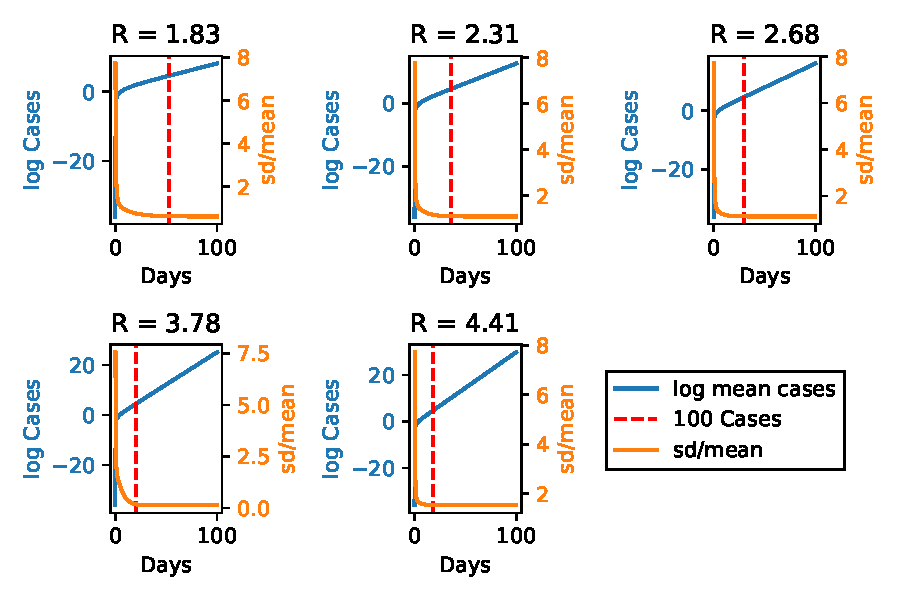
\includegraphics[width = \textwidth]{sig_over_mean_comparison.pdf}
\caption{Plot of the log of the expected number of cases over time (blue curve) for different values of R for the invading VoC, as well as the standard deviation of the number of cases divided by the mean (orange curve). By the time the expected number of cases has reached 100 (dashed red line), the gradient of the standard deviation divided by the mean is approximately zero. Once this has happened, we assume that the number of cases is approximately normally distributed over time, centred on the mean, and hence a deterministic approximation of the epidemic is valid. } 
\label{fig: sig_over_mean}
\end{figure}

\bibliographystyle{plain}
\bibliography{references.bib}
\end{document}


